\documentclass[12pt]{article}
\usepackage{amsmath}
\usepackage{amssymb}
\usepackage[procnames]{listings}
\usepackage{fullpage}
\usepackage{graphicx}
\usepackage{subfigure}
\usepackage{hyperref}
\usepackage{color}
\usepackage{url}

\definecolor{keywords}{RGB}{255,0,80}
\definecolor{comments}{RGB}{0,0,113}
\definecolor{red}{RGB}{80,0,0}
\definecolor{green}{RGB}{0,60,0}
\definecolor{highlightred}{RGB}{255,190,190}
\definecolor{highlightgreen}{RGB}{190,255,190}
\definecolor{highlightwhite}{RGB}{255,255,255}
 
\lstset{language=Python, 
        basicstyle=\ttfamily\small, 
        keywordstyle=\color{keywords},
        commentstyle=\color{comments},
        stringstyle=\color{red},
        showstringspaces=false,
        identifierstyle=\color{green},
        procnamekeys={def,class},
        frame=single,
        breaklines=true}

\title{\textbf{LING 388} \\ Language and Computers: Final Project \\ \emph{Modeling Poetic Dactylic Hexameter}}
\author{Nicholas Wolf}

\begin{document}
\maketitle


%%% Project Description
\section*{Meta-information}
The following files are contained in my project submission:
\begin{description}
\item[code/classify.py] \hfill \\
Interactive classification script. Prompts the user to enter a line of poetry and, if it is valid, returns the line with metrical scansion markings added as diacritics. 
\item[code/data\_processing.py] \hfill \\
Script to process and build a labeled corpus from text files.
\item[code/aeneid\_classifier] \hfill \\
The trained NLTK classifier is written to file with the Python \texttt{pickle} module for later recall. This eliminates the need to re-train the model every time the script is run. 
\item[data/BookOneNoScansion.txt] \hfill \\
Book One of Virgil's Aeneid, Latin \cite{Virgil}.
\item[data/BookOneScansion1\_33.txt] \hfill \\
Lines 1-33 of Book One of Virgil's Aeneid with metrical scansion, Latin \cite{Rodde}.
\end{description}

\section*{Introduction}
My interest in language was sparked by Latin classes I took in high-school. Latin is an interesting language for a number of reasons --- the aspect of it that always fascinated me is the structure of Roman epic poetry. Virgil's \emph{Aeneid}, the 12-book long poem that tells the story of the founding of Rome, uses a rhythmic scheme called dactylic hexameter. \emph{Dactylic hexameter}\footnote{The ``dactylic" in dactylic hexameter comes from the Greek: $\delta  \acute{\alpha} \kappa \tau \upsilon \lambda o \varsigma$, d\'{a}ktylos, ``finger". A poetic dactyl is one long syllable followed by two short syllables just like the human finger is made up of one long bone followed by two short bones!} is a meter that consists of lines made from six bars or ``feet". Each foot can be either a \emph{dactyl}, which contains a long syllable followed by two short syllables (``dum-ditty"), and is marked with the notation: 
\begin{align*}
- \smallsmile \smallsmile
\end{align*}
or a \emph{spondee}, which contains a long syllable followed by another long syllable (``dum-dum"),and is marked as: 
\begin{align*}
- -
\end{align*} 
The only exception to this rule is in the sixth foot, where the last syllable in the line is an anceps syllable. \emph{Anceps} can function as either long or short and are either marked with a $\times$ or left blank. The metrical pattern of a line of dactylic hexameter looks something like:
\begin{align*}
- \smallsmile \smallsmile | - \smallsmile \smallsmile | - -\ | - - \ | \ - \smallsmile \smallsmile | - \times
\end{align*}
Here's an example from the \emph{Aeneid} in which Virgil uses a series of dactyls to express the speed of a running horse:
\begin{center}
q\={ua}dr\u{u}p\u{e} $\vert$ d\={a}nt\u{e} p\u{u} $\vert$ tr\={e}m s\u{o}n\u{i} $\vert$ t\={u} q\u{ua}t\u{i}t $\vert$ \={u}ng\u{u}l\u{a} $\vert$ c\={a}mpum
\end{center}
\begin{center}
``a hoof shakes the crumbling field with a galloping sound"
\end{center}
And another in which he does the opposite --- using a series of spondees to mimic the pounding sound of blacksmiths at work \cite{wiki_dactylic_hexameter}:
\begin{center}
\={i}ll(i) \={i}n $\vert$ t\={e}r s\={e} $\vert$ s\={e} m\={u}l $\vert$ t\={a} v\={i} $\vert$ br\={a}cch\u{i}\u{a} $\vert$ t\={o}llunt
\end{center}
\begin{center}
``take up their arms with great strength one to another"
\end{center}

The second line illustrates something that makes all of this even more complicated --- a phenomenon called elision.  If a word-terminal syllable ends in a vowel and the next word in the line begins with a vowel, the syllable can be completely omitted from the meter and the two words blend together when pronounced. In the line above, `\emph{\={i}ll(i) \={i}nt\={e}r}' would be pronounced as `\emph{\={i}ll\={i}nt\={e}r}'. This is marked by wrapping the omitted vowel in ( ).   

Latin poetry does not normally come with the syllable lengths and meters marked. Presumably, Latin speakers naturally knew how to determine syllable length. It is harder for a non-native speaker to learn how to do. Mainly because the rules for what makes a syllable long or short are really more of suggestions that the author can choose to break for poetic effect.\footnote{I will touch more on these rules when I discuss computationally extracting features from a line of poetry.} This allows the author more freedom for creative expression but also makes metrical scansion more difficult than just learning a set of rules. In my project, I write a computer program that uses a statistical model to scan lines of Latin poetry. I first create a naive Bayesian model to estimate the emission probability distribution of a Hidden Markov Model (HMM). I then find the Viterbi path on the HMM to predict the most likely sequence of syllable lengths for the line of poetry. 

\section*{Building a Corpus}
I obtained two corpora --- a normal copy of Virgil's \emph{Aeneid} (in Latin) \cite{Virgil} and a copy of the first 33 lines of the first book of the \emph{Aeneid} with metrical scansion (also in Latin) \cite{Rodde}. I will refer to them as the non-scanned corpus and the scanned corpus, respectively. As an example, here is the first line from the non-scanned corpus:
\begin{center}
Arma virumque cano, Trojae qui primus ab oris.
\end{center}
And from the scanned corpus
\begin{center}
\={A}rm\u{a} v\u{i}r  $\vert$ \={u}mq\u{ue} c\u{a}  $\vert$  n\={o}, Tr\={oj} $\vert$ \={ae} q\={ui} $\vert$ pr\={i}m\u{u}s \u{a}b $\vert$ \={o}ris 
\end{center}

In order to train the naive Bayes classifier, I needed to build a labeled corpus that contained a list of $(syllable,\ length)$ tuples and preserved the word and line structures from the original text so that I could easily answer questions like ``is this syllable the last one in the line?" when generating feature-sets for the syllables.

The author of the scanned corpus, Daniel Rodde, marked the metrical scansion with accented characters. I was able to extract the syllable lengths from the scanned corpus by iterating over the unicode decomposition of every character in the text --- any decomposition that contained U+0304 (macron, e.g. \={a}) denoted a long syllable and any decomposition that contained U+0306 (breve, e.g. \u{a}) denoted a short one. Elisions were marked at every ``("\footnote{The corpus was pre-processed to remove all of the parenthesis that occurred in the original text.} and in-determinate syllables were marked at the end of every line.

One of the most difficult parts of this project was writing a regular expression to correctly syllabify Latin words. I eventually settled on the regular expression:
\lstinputlisting[breaklines]{re.py}
When passed into \texttt{re.findall(syllable\_pattern, word)}, it returns a list of all the syllables in \texttt{word}.\footnote{The only issue I've noticed with this regular expression is that it has a hard time recognizing the syllable ``tyr".} I used this to break the non-scanned corpus into syllables, and then zipped the array of syllables with the array of syllable lengths from the scanned corpus to create my labeled corpus. 

\section*{Extracting Features}
My next task was building a feature set for all of the syllables in my labeled corpus. In Latin dactylic hexameter, there are four categories of traits that influence syllable length. They are ordered here roughly by the strength with which they contribute to the determination of the length of a syllable. \cite{Farrell1999, Boyd2009} were immensely helpful in choosing these features. 

\begin{enumerate}

\item `Ultima'
\begin{enumerate}
\item The first syllable on a line is always long. 
\item The second to last syllable on a line is always long vowel.
\item The last syllable on a line always has an in-determinant length. 
\end{enumerate}

\item Length by Nature
\begin{enumerate}
\item Word-terminal syllables (i.e. the last syllable in a word) that end in \emph{-o, -i, -u} are usually long. 
\item Word-terminal syllables that end in \emph{-as, -es, -us} are usually long. 
\item Word-terminal syllables that end in \emph{-a, -is} are often short. 
\item Word-terminal syllables that end in \emph{-e} are usually short.
\item Word-terminal syllables that end in \emph{-us} are usually short. 
\item Word-terminal syllables that end in \emph{-am, -em, -um} are usually short. 
\end{enumerate}

\item Length by Position
\begin{enumerate}
\item Vowels that are followed by two consonants are usually long.
\item Vowels that are followed by stop-liquids (e.g. \emph{tr}) are sometimes long.
\item Diphthongs (e.g. \emph{ae}) are usually long. 
\end{enumerate}

\item Ability to Elide
\begin{enumerate}
\item Word-terminal syllables that end in a vowel or \emph{-m} and are followed by a word that begins with a vowel or an \emph{h-} can, but don't have to, elide.
\end{enumerate}

\end{enumerate}

The ways that these features influence the length of a syllable are qualified with words that are frustratingly ambiguous --- words like 'often', 'usually' and 'sometimes'. One of the nice side-effects of building a statistical model to classify the lengths of syllables is that it can estimate the distributions that underlie those fuzzy qualifiers. Another nice side-effect is that training the classifier on a single author's work will produce a sort of fingerprint that captures that author's tendencies to break, bend and ignore rules. 

\section*{Training}
My labeled corpus comprises 33 lines (506 syllables) of poetry. I trained the built-in NLTK naive Bayesian classifier on 75\% of the data and withheld the remaining 25\% for testing.

\section*{Evaluation}
After the classifier was trained, it classified syllables in the test fold with an accuracy of 81.8\% --- baseline performance is 54.0\%\footnote{Every syllable tagged as 'Long'.}. The tendencies of the classifier can be seen in the confusion matrix in Table \ref{ref:naive_confusion}.

\begin{table}[h]
\begin{center}
\begin{tabular}{| r | r | r | r | r |}
\hline
& \textbf{Long} & \textbf{Short} & \textbf{In-determinate} & \textbf{Elision} \\ \hline
\textbf{Long} & 43.7\% & 9.5\% & -- & 0.8\% \\ \hline
\textbf{Short} & 7.1\% & 28.6\% & -- & 0.8\% \\ \hline
\textbf{In-determinate} & -- & -- & 6.3\% & -- \\ \hline
\textbf{Elision} & -- & -- & -- & 3.2\% \\ \hline
\end{tabular}
\caption{Confusion matrix for naive Bayesian classifier (rows = reference).}
\label{ref:naive_confusion}
\end{center}
\end{table}
Below is the output from the classifier on the entire testing set. Green lines are correctly labeled. Red lines are incorrect and illegal dactylic hexameter.
\begin{center}
\colorbox{highlightred}{\={A}RM\u{A} v\u{i}r\={u}mqu\u{e} c\={a}n\={o} Tr\={o}j\={ae} \u{qui} pr\u{i}m\u{u}s \u{a}b \={o}ris}\\ 
\colorbox{highlightred}{\={I}t\u{a}l\u{i}\={a}m f\={a}t\={o} pr\={o}f\u{u}g\u{u}s L\u{a}v\u{i}n\u{a}qu\u{e} v\={e}nit}\\ 
\colorbox{highlightred}{L\={i}t\={o}r\={a} m\={u}l(tum) \={i}l(le) \={e}t t\={e}rr\={i}s j\={a}ct\u{a}t\u{u}s \={e}t \={a}lto}\\ 
\colorbox{highlightred}{V\={i} s\u{u}p\u{e}r\={u}m s\={ae}v\={ae} m\u{e}m\={o}r\={e}m J\={u}n\={o}n\={i}s \u{o}b \={i}ram}\\ 
\colorbox{highlightred}{M\={u}lt\u{a} qu\u{o}(que) \={e}t b\={e}ll\={o} p\={a}ss\u{u}s d\={u}m c\={o}nd\u{e}r\={e}t \={u}rbem}\\ 
\colorbox{highlightgreen}{\={i}nf\={e}r $\vert$ r\={e}tqu\u{e} d\u{e} $\vert$ \={o}s L\u{a}t\u{i} $\vert$ \={o} g\u{e}n\u{u}s $\vert$ \={u}nd\u{e} L\u{a} $\vert$ t\={i}num}\\ 
\colorbox{highlightred}{\={A}lb\u{a}n\u{i}qu\u{e} (pa)tr\={e}s \={a}t(que) \={a}lt\={ae} (moe)n\u{i}\u{a} R\={o}mae}\\ 
\colorbox{highlightred}{M\={u}s\u{a} m\u{i}h\u{i} c\={au}s\={a}s m\u{e}m\={o}r\={a} qu\u{o} n\u{u}m\u{i}n\u{e} l\={ae}so}\\
\end{center}

\section*{Extending the Model}
The naive Bayesian classifier assumes independence between syllables --- the model doesn't consider the lengths of the other syllables in a line when predicting the length of a particular syllable. Even though the classifier is more than 80\% accurate at a syllable level, all but one of the output lines are illegal dactylic hexameter! The problem can be better modeled by a Hidden Markov Model (HMM). Figure \ref{fig:state_transition} represents the state transition diagram for this HMM. 

%%% Figure
\begin{figure}[htb]
\begin{center}
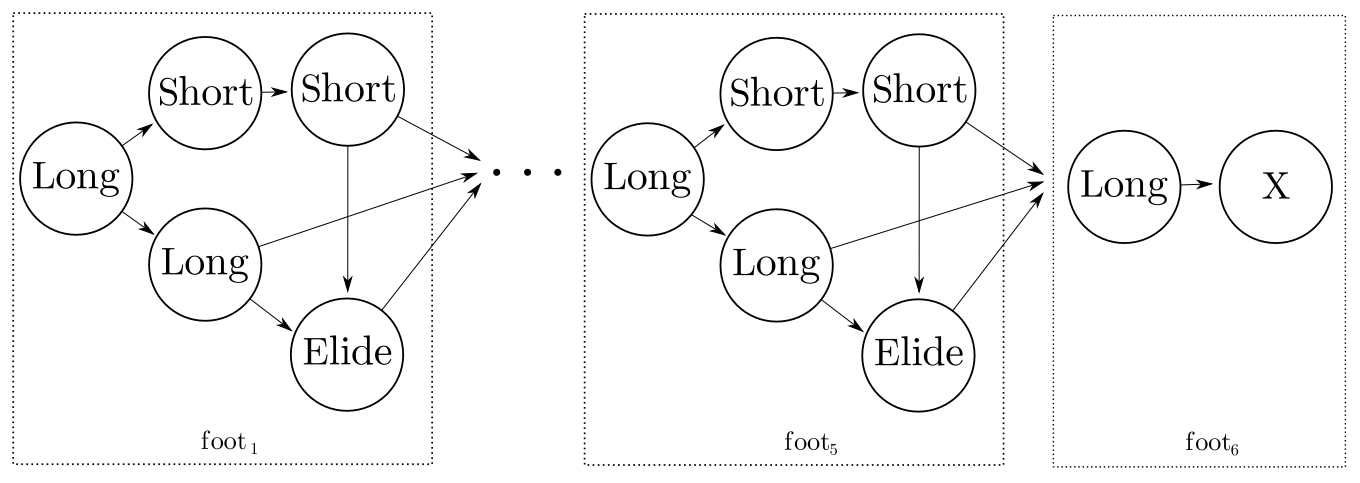
\includegraphics[width=13.5cm]{../figs/graph.png}
\caption{State transition diagram for vowel length in a line of dactylic hexameter.}
\label{fig:state_transition}
\end{center}
\end{figure}

Any path from the long syllable on the left side of the diagram (the first syllable in the line) to the indeterminate ($\times$) syllable on the right side (the last syllable in the line) constitutes a sequence that is a legal line of dactylic hexameter. I assume that the transition probability distribution from any state is uniform over the set of possible next states and the emission probability for each state is given by the naive Bayesian model trained earlier.

Computing the most likely sequence of syllable lengths for a line of poetry is fairly easy --- each foot, except for the last, can have one of four scansions
\begin{gather}
- - \\
- - (elide) \\
- \smallsmile \smallsmile \\
- \smallsmile \smallsmile (elide)
\end{gather}
and the last foot is a given
\begin{align*}
- \times
\end{align*}
so the space of possible paths is actually relatively small ($4^5 = 1024$). For any given line, the space can be further restricted by only considering paths that have a length equal to the number of syllables in the line. A line with 15 syllables, for example, only has 120 different possible metrical sequences. This is a small enough search space that it is not very expensive to compute the log-likelihood of \emph{every} possible path. The path with the smallest negative log-likelihood corresponds to the most likely sequence of syllable lengths. Classifying a line of poetry by calculating the most likely sequence of hidden states in the HMM improves syllable classification accuracy to 85.3\% and (more importantly) ensure that every line of labeled poetry that comes out of the classifier is legal. Below is the output from the new classifier on the entire test set. Green lines are correctly labeled. Non-highlighted lines are incorrect but legal dactylic hexameter.

\begin{center}
\colorbox{highlightwhite}{\={A}RM\u{A} v\u{i}r $\vert$ \={u}mqu\u{e} c\u{a} $\vert$ n\={o} Tr\={o} $\vert$ j\={ae} \u{qui} pr\u{i} $\vert$ m\={u}s \={a}b $\vert$ \={o}ris}\\ 
\colorbox{highlightwhite}{\={I}t\u{a}l\u{i} $\vert$ \={a}m f\={a} $\vert$ t\={o} pr\={o} $\vert$ f\={u}g\u{u}s L\u{a} $\vert$ v\={i}n\u{a}qu\u{e} $\vert$ v\={e}nit}\\ 
\colorbox{highlightwhite}{L\={i}t\={o}r\={a} m\={u}l $\vert$ (tum) \={i}ll\u{e} \u{e}t $\vert$ t\={e}rr\u{i}s j\u{a}c $\vert$ t\={a}t\u{u}s \u{e}t $\vert$ \={a}lto}\\ 
\colorbox{highlightwhite}{V\={i} s\u{u}p\u{e}r $\vert$ \={u}m s\={ae} $\vert$ v\={ae} m\u{e}m\u{o} $\vert$ r\={e}m J\={u} $\vert$ n\={o}n\u{i}s \u{o}b $\vert$ \={i}ram}\\ 
\colorbox{highlightgreen}{M\={u}lt\u{a} qu\u{o} $\vert$ (que) \={e}t b\={e}l $\vert$ l\={o} p\={a}s $\vert$ s\={u}s d\={u}m $\vert$ c\={o}nd\u{e}r\u{e}t $\vert$ \={u}rbem}\\ 
\colorbox{highlightgreen}{\={i}nf\={e}r $\vert$ r\={e}tqu\u{e} d\u{e} $\vert$ \={o}s L\u{a}t\u{i} $\vert$ \={o} g\u{e}n\u{u}s $\vert$ \={u}nd\u{e} L\u{a}t $\vert$ \={i}num}\\ 
\colorbox{highlightgreen}{\={A}lb\={a} $\vert$ n\={i}qu\u{e} p\u{a}t $\vert$ r\={e}s \={a}t $\vert$ (que) \={a}lt\={ae} $\vert$ m\={oe}n\u{i}\u{a} $\vert$ R\={o}mae}\\ 
\colorbox{highlightgreen}{M\={u}s\u{a} m\u{i} $\vert$ h\={i} c\={au} $\vert$ s\={a}s m\u{e}m\u{o} $\vert$ r\={a} qu\u{o} n\u{u} $\vert$ m\={i}n\={e} $\vert$ l\={ae}so}\\
\end{center}
Line-level accuracy has increased by a factor of four and every line is legal dactylic hexameter. 

\section*{Future Work}
There are a few things that could improve the classifier I've built, and a few things that I think would be fun to do with it. 
\begin{enumerate}
\item I would like to construct a larger corpus to train the model on. The current corpus has 506 labeled syllables in it but only 33 lines of poetry. Given the influence that the structure of a line has on the lengths of the syllables in it, 33 is too small of a number to train an accurate model. An additional benefit of having more lines is that it would allow the construction of a prior distribution that could capture a belief in how likely the scansion pattern of a line is (Virgil hardly ever writes lines with only long vowels, for example, so that sequence should have a lower prior probability than others). 
\item The Viterbi algorithm is a dynamic programming approach that reduces the computational complexity of calculating the most likely sequence of states in the HMM from exponential to linear time \cite{Bishop2006a}. While it isn't necessary for the classifier currently, I would like to implement it because it would make it computationally feasible to extend the model to capture dependency between lines, which could be an interesting area of exploration. 
\item I would like to develop a metric for measuring the character of a line of dactylic hexameter (e.g. lines with a lot of long syllables feel slower than lines with a lot of short syllables) so that the way the character of a poem changes over the course of a chapter, section, or book could be visualized. 
\item A foot of dactylic hexameter can be thought of as a four-bar musical phrase where long syllables correspond to half notes and short syllables correspond to quarter notes. I think it would be interesting to run an entire book of the \emph{Aeneid} through the classifier, write the metrical scansion to a MIDI file, and then use it in a musical composition as a rhythm track. 
\item I'm curious to investigate how difficult it would be to extend this model to be able to scan other poetic meters. 
\end{enumerate}
\bibliographystyle{unsrt}
\bibliography{/home/nic/Documents/bibtex/school-nlp-final_project}

%%%% Figure
%\begin{figure}[htb]
%\begin{center}
%\includegraphics[width=12cm]{../figs/FIG}
%\caption{}
%\label{fig:FIG}
%\end{center}
%\end{figure}

%%%% Subfigure
%\begin{figure}[htb]
%\begin{center}
%\subfigure[] {
%	\includegraphics[width=6cm]{../figs/FIG1}
%}
%\subfigure[] {
%	\includegraphics[width=6cm]{../figs/FIG2}
%}
%\caption{}
%\label{fig:SUBFIG}
%\end{center}
%\end{figure}

\end{document}